\chapter{Implementation}\label{ch:implementation}

\section{Preparation}\label{sec:preparation2}

\subsection{Selection of blockchain network}\label{subsec:selection-of-blockchain-network}

As seen in \cref{tab:selection-of-blockchain-network}, the findings in~\cref{sec:voting-systems} can be applied as selection criteria for relevant \gls{Blockchain} networks (see \cref{subsec:comparison-of-turing-complete-blockchains}).
However, some properties mentioned in~\cref{sec:voting-systems} depend entirely on decisions relating to frontend design and code governance rather than the selected \gls{Blockchain}, e.g., whether the software is open-source.
These are displayed in gray in~\cref{tab:selection-of-blockchain-network}.

\begin{table}[H]
    \begin{tabularx}{\textwidth}{bCCCC}
        \hline
        \textbf{Property} & \textbf{Ethereum} & \textbf{Hyperledger Fabric} & \textbf{Polygon} & \textbf{Solana} \\
        \hline
        Auditability & \dblcmark & \dblcmark & \dblcmark & \dblcmark \\
        \hline
        Anonymity & \dblcmark & \cmark & \dblcmark & \cmark  \\
        \hline
        \rowcolor{lightgray}
        Usability & - & - & - & -  \\
        \hline
        \rowcolor{lightgray}
        Accessibility & - & - & - & - \\
        \hline
        Security & \dblcmark & \cmark & \dblcmark & \cmark   \\
        \hline
        Scalability & \xmark & \cmark & \cmark & \cmark  \\
        \hline
        \rowcolor{lightgray}
        Transparency & - & - & - & - \\
        \hline
        Incoercibility & \xmark & \xmark & \xmark & \xmark  \\
        \hline
    \end{tabularx}
    \caption{Comparison of blockchains based on voting system requirements}
    \label{tab:selection-of-blockchain-network}
\end{table}

All four \gls{Blockchain} networks possess most of the necessary properties.
Nevertheless, as shown in \cref{subsec:comparison-of-turing-complete-blockchains}, scalability is a major issue underlying \gls{Blockchain} technology in general.
For instance, even though the Ethereum Foundation is looking to improve Ethereum's protocol further, theoretically enabling it to process up to 100,000 \gls{TPS} in the future, as of the time of this writing, it is not able to process enough transactions to facilitate national elections.
Conversely, other \glspl{Blockchain} compromise on similarly essential features to achieve a higher number of \gls{TPS}, e.g., security or network stability, the latter being an equally important scalability aspect.
Unfortunately, in the absence of a \gls{Blockchain} protocol that satisfies all aspects shown in~\cref{sec:voting-systems}, compromises in our selection process are unavoidable.
Bearing this in mind and looking at \cref{tab:selection-of-blockchain-network}, Polygon is the most logical choice as it runs on top of Ethereum.
Therefore, it automatically benefits from Ethereum's superior security and anonymity, as well as all future improvements made to Ethereum's protocol, while still having an edge in terms of scalability due to its Layer 2 protocol (see~\cref{subsec:comparison-of-turing-complete-blockchains}).

\subsection{Selection of technology stack}\label{subsec:selection-of-tech-stack}

Many frameworks could be used to develop the server- and client-side of a decentralized electronic voting system.
However, we rely on a full Node.js integration due to its non-blocking \gls{IO} to ensure high scalability (see~\cref{subsec:node.js}).
Similarly, given the scalability advantages of monorepos (see~\cref{subsec:nx}), we utilize nx to manage the project's repository.
Additionally, keeping transparency in mind (see~\cref{sec:voting-systems}), an open-source project built with nx is more accessible to other developers as a resource for future research.

We use Next.js as a framework on the client side as it allows for server-side rendering, increasing the application's overall security (see~\cref{subsec:next.js}) and making it \glstext{SEO}-friendly.
Alternatively, we could have chosen to develop the client-side with Nuxt.js, which mimics most of Next.js's server-side and static rendering methods, while using Vue.js instead of React.js.
Nevertheless, Nuxt.js has a smaller community, arguably making React.js the preferable choice.

Although Next.js comes with its own routing framework for API calls, it is reasonable to use a separate framework for requests that handle database and smart contract actions.
Therefore, we utilize Nest.js, which eases the process of following best practices regarding the development of backend applications.
As illustrated in~\cref{subsec:nest.js}, Nest.js is specifically designed with scalability in mind;
moreover, it ensures high readability for developers with either an \gls{OOP} or \gls{FP} background.
Likewise, we handle  database-related aspects of the application using a PostgreSQL database since a broad spectrum of developers should be familiar with a \gls{ORDBMS} and PostgreSQL in particular (see~\cref{subsec:postgresql}).

\section{Setting up the workspace}\label{sec:setting-up-the-workspace}

\subsection{Creating a GitHub repository}\label{subsec:creating-a-git-repository}

\begin{figure}[h]
    \centering
    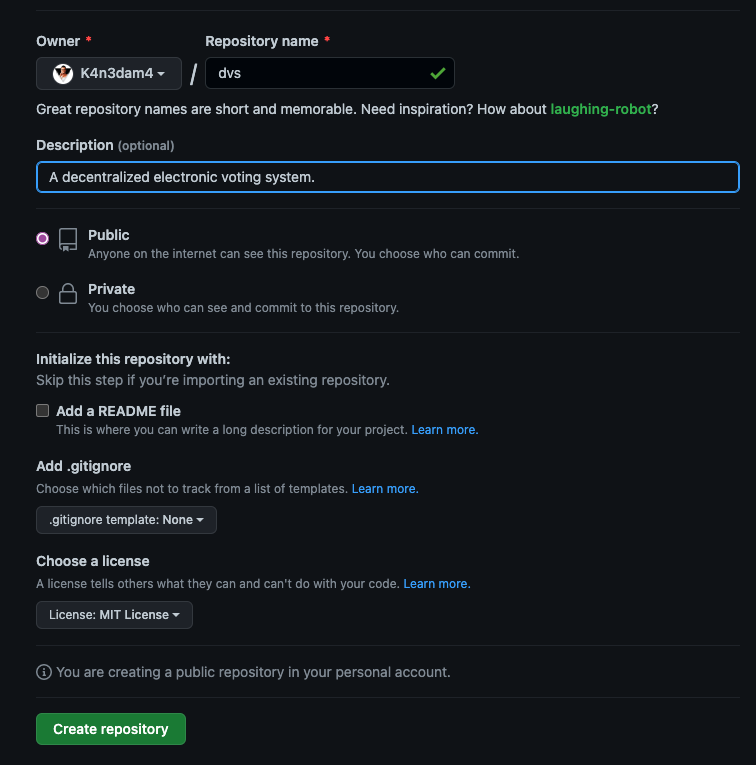
\includegraphics[scale=0.4]{boehm-initializing-repository}
    \caption[Creating a Github repository]{Creating a Github repository. Screenshot taken by author}
    \label{fig:initializing-repository}
\end{figure}

For the reasons discussed in~\cref{subsec:versioning}, the first step in the development process is the creation of a GitHub repository.
As seen in~\cref{fig:initializing-repository}, we change the license from \emph{None} to \emph{MIT License} to make this project available to the scientific community as a resource for further research.
Next, the repository is initialized, containing neither a README nor a .gitignore file, as these are automatically created by nx (see~\cref{subsec:creating-a-monorepo-using-nx}).

\subsection{Creating a monorepo using nx}\label{subsec:creating-a-monorepo-using-nx}

Creating a monorepo with nx is a straightforward process using the nx-provided executable package \emph{create-nx-workspace} with \gls{npx}.

\begin{figure}[h]
    \begin{subfigure}[b]{\textwidth}
        \centering
        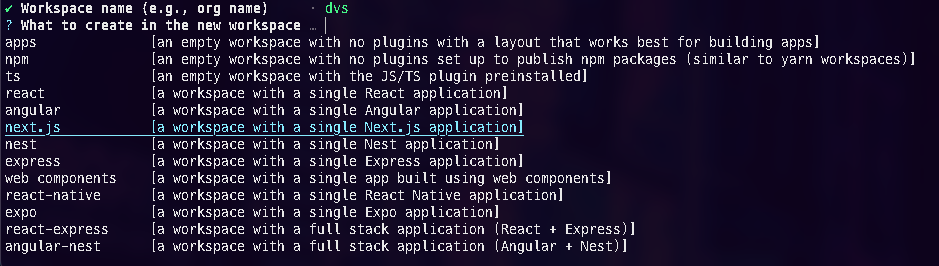
\includegraphics[width=\textwidth]{nx-workspace-options-0}
        \caption{Options for app templates nx can automatically build during initialization}
        \label{fig:nx-workspace-options-0}
    \end{subfigure}
    \begin{subfigure}[b]{0.5\textwidth}
        \centering
        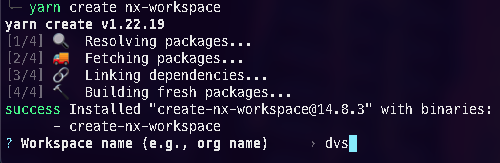
\includegraphics[width=\textwidth, height=85px]{nx-workspace-name}
        \caption{Naming the workspace}
        \label{fig:nx-workspace-name}
    \end{subfigure}
    \begin{subfigure}[b]{0.5\textwidth}
        \centering
        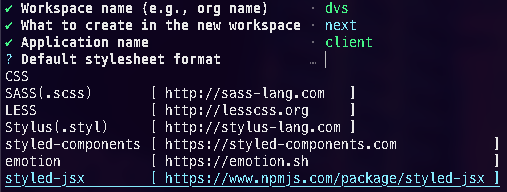
\includegraphics[width=\textwidth]{nx-workspace-options-1}
        \caption{Default style format options}
        \label{fig:nx-workspace-options-1}
    \end{subfigure}
    \caption[Setting up a nx workspace]{Setting up a nx workspace. Screenshots taken by author}
    \label{fig:setting-up-nx-workspace}
\end{figure}

After initiating the process by typing \mintinline{text}{yarn create nx-workspace} in the terminal, nx allows developers to name (see~\cref{fig:nx-workspace-name}) the project.
Next, developers are offered several template options for an initial application nx then automatically adds to the workspace (see~\cref{fig:nx-workspace-options-0,fig:nx-workspace-options-1}).
Given these options, we initialize the workspace with a Next.js application for the client side of the voting system.
Alternatively, we could initialize it containing a Nest.js application, but the order in which client and server applications are added to the workspace is irrelevant in this context.

\section{Setting up the backend}\label{sec:setting-up-a-nest.js-backend}

\subsection{Creating a Nest.js application}\label{subsec:creating-a-nest.js-application}

The installation of a plugin with \mintinline[breaklines]{text}{yarn add -D @nrwl/nest} is necessary to let nx handle the installation process of the Nest.js application.
After installing the plugin, we add a new Nest.js application to the workspace using the \mintinline[breaklines]{text}{nx g @nrwl/nest:app api} command, where \emph{server} is the name given to the application.

To maintain scalability, we combine Nest.js's modular design with nx's \emph{libs} directories, meaning backend controllers and services are kept as separate modules in \emph{libs/api} rather than the \emph{apps/server} directory.
As mentioned in~\cref{subsec:nx}, modularizing code within the \emph{libs} directory makes it reusable in all workspace applications sharing the same scope.
Hence, all future applications that might be added to the project will also be able to access that code if needed, thus making it easier to adhere to \gls{DRY} principles.

\subsection{Creating a PostgreSQL database}\label{subsec:creating-a-postgresql-database}

To handle database entries, we create a new Nest.js module, \emph{prisma}, in the \emph{libs/api} folder.
Then, we install Prisma as a devDependency with \mintinline[breaklines]{text}{yarn add -D prisma}, which provides basic tooling for databases, such as creating type-safe schemas, a built-in migration system, and a \gls{GUI} to display and edit database entries.
Following the installation process, we create a docker-compose.yml, enabling the application to run dockerized PostgreSQL databases during development, test, and production builds (see listing~\ref{lst:docker-compose.yml}).

\codeFromFile{yaml}{code_snippets/docker-compose.yml}{Docker-compose.yml used in the prisma module}{Docker-compose.yml used in the prisma module}{lst:docker-compose.yml}

Having created a docker-compose file, along with the commands necessary to run the database in the prisma module’s project.json and the project’s package.json, we can add a core Nest.js module (see listing~\ref{lst:core-module}).
The core module makes configurations such as the database \gls{URL} available throughout the Nest.js application.
We then proceed with connecting our Nest.js application to the database through the prisma service (see listing~\ref{lst:prisma-service}) using the \gls{URL} from the core module.

\codeFromFile{ts}{code_snippets/nest-core-module.ts}{Core module}{Core module}{lst:core-module}
\codeFromFile{ts}{code_snippets/nest-prisma-service.ts}{Prisma service}{Prisma service}{lst:prisma-service}

\section{Preparing for smart contract development}\label{sec:preparing-for-smart-contract-development}

\subsection{Setting up our IDE}\label{subsec:setting-up-our-ide}

Since our local \gls{IDE} (IntelliJ IDEA) does not natively support Solidity, our first step is to install the \emph{IntelliJ Solidity} plugin.
After installing the plugin, the \gls{IDE} should be able to recognize Solidity files (.sol) and provide us with basic syntax highlighting.
Unfortunately, the plugin does not provide autocomplete, making for an unpleasant development experience.

It should be noted that this is a problem specific to our preferred \gls{IDE}.
Developers running another \glsfirst{IDE}, such as VSCode or Atom, should be better equipped to write their Solidity code locally.
Nevertheless, since we do neither wish to switch to VSCode nor Atom, we will use the Remix \gls{IDE} to develop our smart contract online.

\subsection{Setting up Remix}\label{subsec:setting-up-remix}

As mentioned in \cref{subsec:remix-ide}, Remix Project provides us with an \glsfirst{IDE} and tools to deploy and debug our written code.
Although, we will later copy the code to our local workspace (see~\cref{subsec:setting-up-local-hardhat-project}) to use the contract's \gls{ABI} in the rest of our project.

\begin{figure}[h]
    \centering
    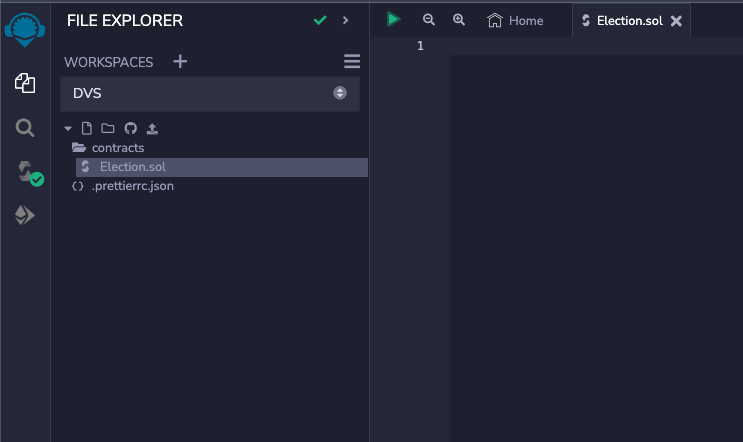
\includegraphics[width=\textwidth]{boehm-remix-startup}
    \caption[Setting up Remix]{Setting up Remix. Screenshot taken by author}
    \label{fig:remix-setup}
\end{figure}

Opening Remix \gls{IDE} for the first time, we see several example files in the \emph{contracts} and the \emph{scripts} directory.
So after deleting those, we create a new file in the \emph{contracts} folder called \emph{Election.sol} (see~\cref{fig:remix-setup}).

\subsection{Setting up local Hardhat project}\label{subsec:setting-up-local-hardhat-project}

Since our backend will depend on the \gls{ABI} of our written contract, we still need to set up a local project.
First, we use the nx command \mintinline{text}{nx g lib smart-contracts} to create a new nx library.
Afterward, we need to install the necessary Hardhat dependencies in our project's root directory

\begin{minted}{shell-session}
    yarn add -D hardhat @nomicfoundation/hardhat-toolbox
\end{minted}

and chai matchers to enable local testing of our election contract, as well as typechain, since we are going to need typed interfaces of our contracts

\begin{minted}[breaklines, style=material]{shell-session}
    yarn add -D @nomicfoundation/hardhat-chai-matchers @types/chai @types/mocha typechain @types/typechain
\end{minted}

After installing all necessary dependencies, we configure Hardhat and tell it to run within its directory in \emph{libs/smart-contracts} by creating a \emph{hardhat.config.ts} (see listing~\ref{lst:hardhat-config}) and adding nx commands for testing and compilation to the library's \emph{project.json} (see listing~\ref{lst:hardhat-project.json}).

\codeFromFile{ts}{code_snippets/hardhat-config.ts}{Hardhat config}{Hardhat config}{lst:hardhat-config}
\codeFromFile{json}{code_snippets/hardhat-project.json}{Hardhat project.json}{Hardhat project.json}{lst:hardhat-project.json}

\section{Smart contract}\label{sec:smart-contract}

To begin writing the smart contract, we will later deploy when admins create an election; we switch to Remix \gls{IDE} and open the \emph{Election.sol} file we created earlier.

\subsection{Selecting a Solidity compiler and language version}\label{subsec:selecting-a-solidity-compiler-and-language-version}

In contrast to code written in JavaScript, Solidity compiles to bytecode.
Hence, we need to start every .sol file we create with a \emph{compiler directive}, known as \emph{version pragma}~\autocite[135]{antonopoulos_mastering_2019}, that specifies the compiler and language version our contract expects

\begin{minted}{solidity}
// SPDX-License-Identifier: MIT
pragma solidity ^0.8.17;
\end{minted}

Our contract will be using Solidity 0.8.17, as well as higher minor versions, e.g., 0.8.20.

\subsection{Importing Ownable.sol}\label{subsec:impotring-ownable.sol}

Since some functions in the contract will only accept transactions from the admin address that created the election, we also import \emph{@openzeppelin/contracts/access/Ownable.sol} into our contract's context

\begin{minted}{solidity}
// SPDX-License-Identifier: MIT
pragma solidity ^0.8.17;
import "@openzeppelin/contracts/access/Ownable.sol";
\end{minted}

The OpenZeppelin library is a collection of reusable smart contracts that include operations commonly needed when developing smart contracts.
In this case, \emph{Ownable.sol} provides a basic ownership model for our contract, including functions for checking its current owner and transferring ownership to other admins.

\subsection{Defining the contract's structs}\label{subsec:defining-the-contracts-structs}

% use c++ instead of solidity to avoid messed up highlighting
\codeFromFile{sol}{code_snippets/election-step1.sol}{Defining the contract's structs}{Defining the contract's structs}{lst:election-step1.sol}

Since the data pertaining to an election can be split up into information about its candidates, voters and result, we use the struct data type to define how this data will look (see listing~\ref{lst:election-step1.sol}).

\subsection{Defining the contract's states, constructor and modifiers}\label{subsec:defining-the-contract's-states-constructor-and-modifiers}

\codeFromFile{sol}{code_snippets/election-step2.sol}{Defining the contract's states, constructor and modifiers}{Defining the contract's states, constructor and modifiers}{lst:election-step2.sol}

\subsubsection{States}

Subsequently, as shown in listing~\ref{lst:election-step2.sol}, we use these data structures to define the contract's states: 

\begin{enumerate}
    \item The election's name
    \item The expiration timestamp
    \item A mapping for all registered voters, which acts as a hash lookup table iterable with a voter's wallet address~\autocite[137]{antonopoulos_mastering_2019}
    \item An array of the election's candidates
    \item An array of the result
\end{enumerate}

In elections conducted on the blockchain, having a dedicated state holding the election's expiration is essential.
Again, as discussed in~\cref{subsec:blocks}, once a transaction has been saved on the blockchain, it can not be deleted.
Thus, the only possible way to prevent people from voting once an election has expired or an election official has closed it, is to change one of the contract's states to a value that will be checked by its functions before executing them.

\subsubsection{Constructor}

As in other programming languages, a contract's constructor is called only once when a new contract instance is created on the blockchain.
Hence, our constructor accepts three arguments, the election's name, its candidates, and its expiration timestamp, which will be parsed to the contract during deployment (see listing~\ref{lst:election-step2.sol}).

\subsubsection{Modifiers}

The last thing we do before writing the contract's functions is to create a modifier that checks the value saved in the \emph{expires} state against the global variable \emph{block.timestamp}, which is exposed by the \gls{EVM}.
Since every transaction, including transactions that would change the contracts states, have to be added to a block, and each block has a timestamp, we can prevent successful state changes by adding the \emph{checkExpired} modifier to selected functions.

\subsection{Contract functions}\label{subsec:contract-functions}





